% !TEX TS-program = xelatex
% !BIB program = bibtex
% !TeX spellcheck = ru_RU
% !TEX root = talk.tex

\documentclass
  [ russian
  , aspectratio=169 % Для защит онлайн лучше использовать разрешение не 4х3
  ] {beamer}

%%% PDF settings
\pdfvariable minorversion 7 % Set PDF version to 1.7.

%%% Fonts and language setup.
\usepackage{polyglossia}
% Setup fonts.
\usepackage{fontspec}
\setmainfont{CMU Serif}
\setsansfont{CMU Sans Serif}
\setmonofont{CMU Typewriter Text}

\usepackage{microtype} % Add fancy-schmancy font tricks

\usepackage{xcolor} % Add colors support.

%% Math
\usepackage{amsmath, amsfonts, amssymb, amsthm, mathtools} % Advanced math tools.
\usepackage{thmtools}
\usepackage{unicode-math} % Allow TTF and OTF fonts in math and allow direct typing unicode math characters.
\unimathsetup{
    warnings-off={
            mathtools-colon,
            mathtools-overbracket
        }
}
\setmathfont{Latin Modern Math} % default
\setmathfont[range={\setminus,\varnothing,\smashtimes}]{Asana Math}

%%% Images
\usepackage{graphicx}
\graphicspath{{figures/}}
\usepackage{import}

%%% Polyglossia setup after (nearly) everything as described in documentation.
\setdefaultlanguage{russian}
\setotherlanguage{english}

\usepackage{csquotes}

%%% Custom commands
\newcommand{\R}{\mathbb{R}}
\newcommand{\N}{\mathbb{N}}
\newcommand{\Z}{\mathbb{Z}}
\newcommand{\Q}{\mathbb{Q}}
\newcommand{\C}{\mathbb{C}}
\newcommand{\id}{\mathrm{id}}
\AtBeginDocument{\renewcommand{\leq}{\leqslant}}
\AtBeginDocument{\renewcommand{\geq}{\geqslant}}
\AtBeginDocument{\renewcommand{\Re}{\operatorname{Re}}}
\AtBeginDocument{\renewcommand{\Im}{\operatorname{Im}}}
\AtBeginDocument{\renewcommand{\phi}{\varphi}}
\AtBeginDocument{\renewcommand{\epsilon}{\varepsilon}}

%%% theorem-like envs
\theoremstyle{definition}

\declaretheoremstyle[spaceabove=0.5\topsep,
    spacebelow=0.5\topsep,
    headfont=\bfseries\sffamily,
    bodyfont=\normalfont,
    headpunct=.,
    postheadspace=5pt plus 1pt minus 1pt]{myStyle}
\declaretheoremstyle[spacebelow=\topsep,
    headfont=\bfseries\sffamily,
    bodyfont=\normalfont,
    headpunct=.,
    postheadspace=5pt plus 1pt minus 1pt,]{myStyleWithFrame}
\declaretheoremstyle[spacebelow=\topsep,
    headfont=\bfseries\sffamily,
    bodyfont=\normalfont,
    headpunct=.,
    postheadspace=5pt plus 1pt minus 1pt,
    qed=\blacksquare]{myProofStyleWithFrame}

\usepackage[breakable]{tcolorbox}
\tcbset{sharp corners=all, colback=white}
% \tcolorboxenvironment{theorem}{}
% \tcolorboxenvironment{theorem*}{}
% \tcolorboxenvironment{axiom}{}
% \tcolorboxenvironment{assertion}{}
% \tcolorboxenvironment{lemma}{}
% \tcolorboxenvironment{proposition}{}
% \tcolorboxenvironment{corollary}{}
% \tcolorboxenvironment{definition}{}
% \tcolorboxenvironment{proofReplace}{toprule=0mm,bottomrule=0mm,rightrule=0mm, colback=white, breakable }

\declaretheorem[name=Теорема, style=myStyleWithFrame]{theorem}
\declaretheorem[name=Теорема, numbered=no, style=myStyleWithFrame]{theorem*}
\declaretheorem[name=Аксиома, sibling=theorem, style=myStyleWithFrame]{axiom}
\declaretheorem[name=Преположение, sibling=theorem, style=myStyleWithFrame]{assertion}
\declaretheorem[name=Лемма, style=myStyleWithFrame]{lemma}
\declaretheorem[name=Предложение, sibling=theorem, style=myStyleWithFrame]{proposition}
\declaretheorem[name=Следствие, numberwithin=theorem, style=myStyleWithFrame]{corollary}

\declaretheorem[name=Определение, style=myStyleWithFrame]{definition}
\declaretheorem[name=Свойство, style=myStyle]{property}
\declaretheorem[name=Свойства, numbered=no, style=myStyle]{propertylist}

\declaretheorem[name=Пример, style=myStyle]{example}
\declaretheorem[name=Замечание, numbered=no, style=myStyle]{remark}

\declaretheorem[name=Доказательство, numbered=no, style=myProofStyleWithFrame]{proofReplace}
\renewenvironment{proof}[1][\proofname]{\begin{proofReplace}}{\end{proofReplace}}
% \declaretheorem[name=Доказательство, numbered=no, style=myProofStyleWithFrame]{longProof}

%%% Memoir settings
\chapterstyle{ger}
\setlength{\headheight}{2\baselineskip}

%%% HyperRef
\usepackage{hyperref}

\setbeamertemplate{itemize items}[circle]
\setbeamertemplate{enumerate items}[circle]

\newcommand\blfootnote[1]{%
	\begingroup
	\renewcommand\thefootnote{}\footnote{#1}%
	\addtocounter{footnote}{-1}%
	\endgroup
}

\makeatletter

%!TEX root = vkr.tex

%% Параметры заполнения титульного листа
\usepackage{xkeyval}

%% Русскоязычный вариант
\define@key[ru]{mytitle}{chair}{\def\my@title@chair@ru{#1}}
\define@key[ru]{mytitle}{title}{\def\my@title@title@ru{#1}}
\define@key[ru]{mytitle}{group}{\def\my@title@group@ru{#1}}
\define@key[ru]{mytitle}{author}{\def\my@title@author@ru{#1}}
\define@key[ru]{mytitle}{supervisor}{\def\my@title@supervisor@ru{#1}}
\define@key[ru]{mytitle}{supervisorPosition}{\def\my@title@supervisorPosition@ru{#1}}
\define@key[ru]{mytitle}{reviewer}{\def\my@title@reviewer@ru{#1}}
\define@key[ru]{mytitle}{reviewerPosition}{\def\my@title@reviewerPosition@ru{#1}}
\define@key[ru]{mytitle}{consultant}{\def\my@title@consultant@ru{#1}}
\define@key[ru]{mytitle}{consultantPosition}{\def\my@title@consultantPosition@ru{#1}}
\define@key[ru]{mytitle}{year}{\def\my@title@year@ru{#1}}
\define@key[ru]{mytitle}{specialty}{\def\my@title@specialty@ru{#1}}
\define@key[ru]{mytitle}{programme}{\def\my@title@programme@ru{#1}}
\define@key[ru]{mytitle}{profile}{\def\my@title@profile@ru{#1}}
\define@choicekey*[ru]{mytitle}{type}{coursework,practice,prediploma,master,bachelor,production}{\def\my@title@type@ru{#1}}
\define@choicekey*[ru]{mytitle}{kind}{solution,experiment,production,comparison,theoretical}{\def\my@title@kind@ru{#1}}

%% Англоязычный вариант
\define@key[en]{mytitle}{chair}{\def\my@title@chair@en{#1}}
\define@key[en]{mytitle}{title}{\def\my@title@title@en{#1}}
\define@key[en]{mytitle}{group}{\def\my@title@group@en{#1}}
\define@key[en]{mytitle}{author}{\def\my@title@author@en{#1}}
\define@key[en]{mytitle}{supervisor}{\def\my@title@supervisor@en{#1}}
\define@key[en]{mytitle}{supervisorPosition}{\def\my@title@supervisorPosition@en{#1}}
\define@key[en]{mytitle}{reviewer}{\def\my@title@reviewer@en{#1}}
\define@key[en]{mytitle}{reviewerPosition}{\def\my@title@reviewerPosition@en{#1}}
\define@key[en]{mytitle}{consultant}{\def\my@title@consultant@en{#1}}
\define@key[en]{mytitle}{consultantPosition}{\def\my@title@consultantPosition@en{#1}}
\define@key[en]{mytitle}{year}{\def\my@title@year@en{#1}}
\define@key[en]{mytitle}{specialty}{\def\my@title@specialty@en{#1}}
\define@key[en]{mytitle}{programme}{\def\my@title@programme@en{#1}}
\define@key[en]{mytitle}{profile}{\def\my@title@profile@en{#1}}
\define@choicekey*[en]{mytitle}{type}{coursework,practice,prediploma,master,bachelor}{\def\my@title@type@en{#1}}
\define@choicekey*[en]{mytitle}{kind}{solution,experiment,production,comparison,theoretical}{\def\my@title@kind@en{#1}}

\newcommand{\filltitle}[2]{
    %% Значения по умолчанию для обоих языков
    \ifthenelse{\equal{#1}{ru}}
    {
        \presetkeys[#1]{mytitle}{
            year = {\the\year},
            type = {practice},
            reviewer = {},
            consultant = {},
            profile = {}
        }{}
    }
    {}
    \ifthenelse{\equal{#1}{en}}
    {
        \presetkeys[#1]{mytitle}{
            year = {\the\year},
            type = {practice},
            reviewer = {},
            consultant = {},
            profile = {}
        }{}
    }
    {}
    \setkeys[#1]{mytitle}{#2}
}


% !TeX spellcheck = ru_RU
% !TEX root = vkr.tex

%% Если что-то забыли, при компиляции будут ошибки Undefined control sequence \my@title@<что забыли>@ru
%% Если англоязычная титульная страница не нужна, то ее можно просто удалить.
\filltitle{ru}{
	%% Актуально только для курсовых/практик. ВКР защищаются не на кафедре а в ГЭК по направлению,
	%%   и к моменту защиты вы будете уже не в группе.
	chair              = {Кафедра системного программирования},
	group              = {21.Б10-мм},
	%
	%% Макрос filltitle ненавидит пустые строки, поэтому обязателен хотя бы символ комментария на строке
	%% Актуально всем.
	title              = {Разработка инфраструктуры для сборки проектов с открытым исходным кодом для архитектуры \riscv{}},
	%
	%% Здесь указывается тип работы. Возможные значения:
	%%   production - производственная практика;
	%%   coursework - отчёт по курсовой работе;
	%%   practice - отчёт по учебной практике;
	%%   prediploma - отчёт по преддипломной практике;
	%%   master - ВКР магистра;
	%%   bachelor - ВКР бакалавра.
	type               = {practice},
	%
	%% Здесь указывается вид работы. От вида работы зависят критерии оценивания.
	%%   solution - <<Решение>>. Обучающемуся поручили найти способ решения проблемы в области разработки программного обеспечения или теоретической информатики с учётом набора ограничений.
	%%   experiment - <<Эксперимент>>. Обучающемуся поручили изучить возможности, достоинства и недостатки новой технологии, платформы, языка и т. д. на примере какой-то задачи.
	%%   production - <<Производственное задание>>. Автору поручили реализовать потенциально полезное программное обеспечение.
	%%   comparison - <<Сравнение>>. Обучающемуся поручили сравнить несколько существующих продуктов и/или подходов.
	%%   theoretical - <<Теоретическое исследование>>. Автору поручили доказать какое-то утверждение, исследовать свойства алгоритма и т.п., при этом не требуя написания кода.
	kind               = {experiment},
	%
	author             = {Пономарев Николай Алексеевич},
	%
	%% Актуально только для ВКР. Указывается код и название направления подготовки. Типичные примеры:
	%%   02.03.03 <<Математическое обеспечение и администрирование информационных систем>>
	%%   02.04.03 <<Математическое обеспечение и администрирование информационных систем>>
	%%   09.03.04 <<Программная инженерия>>
	%%   09.04.04 <<Программная инженерия>>
	%% Те, что с 03 в середине --- бакалавриат, с 04 --- магистратура.
	specialty          = {02.03.03 <<Математическое обеспечение и администрирование информационных систем>>},
	%
	%% Актуально только для ВКР. Указывается шифр и название образовательной программы. Типичные примеры:
	%%   СВ.5006.2017 <<Математическое обеспечение и администрирование информационных систем>>
	%%   СВ.5162.2020 <<Технологии программирования>>
	%%   СВ.5080.2017 <<Программная инженерия>>
	%%   ВМ.5665.2019 <<Математическое обеспечение и администрирование информационных систем>>
	%%   ВМ.5666.2019 <<Программная инженерия>>
	%% Шифр и название программы можно посмотреть в учебном плане, по которому вы учитесь.
	%% СВ.* --- бакалавриат, ВМ.* --- магистратура. В конце --- год поступления (не обязательно ваш, если вы были в академе/вылетали).
	programme          = {СВ.5006.2019 <<Математическое обеспечение и администрирование информационных систем>>},
	%
	%% Актуально только для ВКР, только для матобеса и только 2017-2018 годов поступления. Указывается профиль подготовки, на котором вы учитесь.
	%% Названия профилей можно найти в учебном плане в списке дисциплин по выбору. На каком именно вы, вам должны были сказать после второго курса (можно уточнить в студотделе).
	%% Вот возможные вариканты:
	%%   Математические основы информатики
	%%   Информационные системы и базы данных
	%%   Параллельное программирование
	%%   Системное программирование
	%%   Технология программирования
	%%   Администрирование информационных систем
	%%   Реинжиниринг программного обеспечения
	% profile            = {Системное программирование},
	%
	%% Актуально всем.
	%supervisorPosition = {проф. каф. СП, д.ф.-м.н., проф.}, % Терехов А.Н.
	supervisorPosition = {старший преподаватель Кафедры\\системного программирования}, % Григорьев С.В.
	supervisor         = {Я.~А.~Кириленко},
	%
	%% Актуально только для практик и курсовых. Если консультанта нет, закомментировать или удалить вовсе.
	% consultantPosition = {должность ООО <<Место работы>>, степень,},
	% consultant         = {К.~К.~Консультант},
	%
	%% Актуально только для ВКР.
	% reviewerPosition   = {должность ООО <<Место работы>> степень},
	% reviewer           = {Р.~Р.~Рецензент},
}

% \filltitle{en}{
%     chair              = {Advisor's chair},
%     group              = {ХХ.BХХ-mm},
%     title              = {Template for SPbU qualification works},
%     type               = {practice},
%     author             = {FirstName Surname},
%     %
%     %% Possible choices:
%     %%   02.03.03 <<Software and Administration of Information Systems>>
%     %%   02.04.03 <<Software and Administration of Information Systems>>
%     %%   09.03.04 <<Software Engineering>>
%     %%   09.04.04 <<Software Engineering>>
%     %% Те, что с 03 в середине --- бакалавриат, с 04 --- магистратура.
%     specialty          = {02.03.03 ``Software and Administration of Information Systems''},
%     %
%     %% Possible choices:
%     %%   СВ.5006.2017 <<Software and Administration of Information Systems>>
%     %%   СВ.5162.2020 <<Programming Technologies>>
%     %%   СВ.5080.2017 <<Software Engineering>>
%     %%   ВМ.5665.2019 <<Software and Administration of Information Systems>>
%     %%   ВМ.5666.2019 <<Software Engineering>>
%     programme          = {СВ.5006.2019 ``Software and Administration of Information Systems''},
%     %
%     %% Possible choices:
%     %%   Mathematical Foundations of Informatics
%     %%   Information Systems and Databases
%     %%   Parallel Programming
%     %%   System Programming
%     %%   Programming Technology
%     %%   Information Systems Administration
%     %%   Software Reengineering
%     % profile            = {Software Engineering},
%     %
%     %% Note that common title translations are:
%     %%   кандидат наук --- C.Sc. (NOT Ph.D.)
%     %%   доктор ... наук --- Sc.D.
%     %%   доцент --- docent (NOT assistant/associate prof.)
%     %%   профессор --- prof.
%     supervisorPosition = {Sc.D, prof.},
%     supervisor         = {S.S. Supervisor},
%     %
%     consultantPosition = {position at ``Company'', degree if present},
%     consultant         = {C.C. Consultant},
%     %
%     reviewerPosition   = {position at ``Company'', degree if present},
%     reviewer           = {R.R. Reviewer},
% }


\newcommand{\academicGroup}{\my@title@group@ru}
\newcommand{\advisorChair}{\my@title@chair@ru}
% То, что в квадратных скобках, отображается внизу по центру каждого слайда.
\title[Lamagraph: Транслятор в Interaction Nets]{\my@title@title@ru}
% То, что в квадратных скобках, отображается в левом нижнем углу.
\author[\my@title@author@ru]{\my@title@author@ru, группа \academicGroup}
\institute[СПбГУ]{}
\date[25 апреля 2025 г.]{}
\newcommand{\supervisor}{\my@title@supervisor@ru}
\newcommand{\supervisorPosition}{\my@title@supervisorPosition@ru}
\newcommand{\consultant}{\my@title@consultant@ru}
\newcommand{\consultantPosition}{\my@title@consultantPosition@ru}
\newcommand{\reviewer}{\my@title@reviewer@ru}
\newcommand{\reviewerPosition}{\my@title@reviewerPosition@ru}
\newcommand{\defenseYear}{\my@title@year@ru}

\makeatother
\begin{document}
{
\setbeamertemplate{footline}{}
% Лого университета или организации, отображается в шапке титульного листа
\begin{frame}
    
\includegraphics[width=1.4cm]{figures/герб_серый.png}
    \vspace{-35pt}
    \hspace{-10pt}
    \begin{center}
        \begin{tabular}{c}
            \scriptsize{Санкт-Петербургский государственный университет} \\
            \scriptsize{\advisorChair}
        \end{tabular}
        \titlepage
    \end{center}

    \btVFill

    {\scriptsize
        % У научного руководителя должна быть указана научная степень
        \textbf{Научный руководитель:} \supervisorPosition~\supervisor \\
        % Консультанта может и не быть. Должна быть указана должность или ученая степень
        % \textbf{Консультант:}  \consultantPosition~\consultant \\
        % Для учебной практики не обязателен. Должна быть указана должность или ученая степень
        \textbf{Рецензент:} \reviewerPosition~\reviewer \\
    }
    \makeatother
    \begin{center}
        \vspace{5pt}
        \scriptsize{Санкт-Петербург\\ \defenseYear}
    \end{center}
\end{frame}
}

\begin{frame}{Введение}

    \begin{itemize}
        \item Задачи искусственного интеллекта и анализа графов влекут за собой нерегулярный параллелизм
        \item Традиционные архитектуры плохо справляются с нерегулярным параллелизмом $\implies$~требуются специализированные ускорители
        \item \INs{}~--- модель вычислений, которой естествен нерегулярный параллелизм
        \item Существуют программные реализации \INs{}, однако попыток реализовать ускоритель на её основе пока не предпринималось
    \end{itemize}

\end{frame}

\begin{frame}{\Lamagraph{}}

    Проект \Lamagraph{} исследует возможности по разработке
    \begin{itemize}
        \item параметризуемого многоядерного сопроцессора на основе \INs{}
        \item ML-подобного функционального языка для программирования сопроцессора
    \end{itemize}
    \begin{center}
        \includegraphics[width=\linewidth]{figures/lamagraph-big-horiz.pdf}
    \end{center}

\end{frame}

\begin{frame}{Состояние проекта}

    Проект на первом этапе: разработка минимальной инфраструктуры для создания ускорителей на основе Interaction Nets

    \vspace{1em}

    На данном этапе от проекта ожидается следующее
    \begin{itemize}
        \item Приоритизация получения полнофункционального прототипа, содержащего все компоненты
        \item Использование единого стека технологий: Clash $\implies$ Haskell
        \item Возможность анализа результатов каждого этапа работы
    \end{itemize}

\end{frame}

\begin{frame}
    \frametitle{Постановка задачи}

    \textbf{Целью} работы является разработка транслятора модельного функционального языка в \INs{}
    \vspace{1em}

    \textbf{Задачи}:
    \begin{enumerate}
        \item Реализовать интерпретатор модельного ML-подобного языка
              \begin{itemize}
                  \item Фронтенд транслятора
                  \item Интерпретатор обогащенного $\lambda$-исчисления
              \end{itemize}
        \item Реализовать транслятор $\lambda$-исчисления в \INs{}
        \item Реализовать интерпретатор \INs{}, поддерживающий сбор метрик исполнения
    \end{enumerate}

\end{frame}

\begin{frame}
    \frametitle{Реализация}

    \begin{center}
        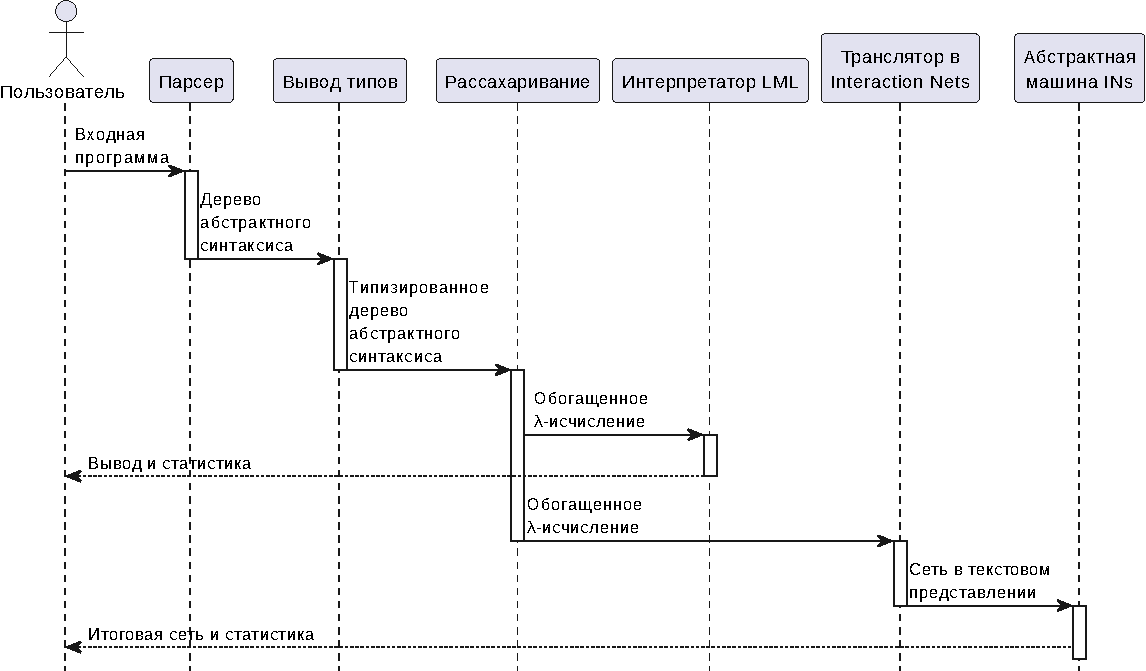
\includegraphics[width=0.8\linewidth]{figures/using.pdf}
    \end{center}

\end{frame}

\begin{frame}{Фронтенд и интерпретатор LamagraphML}

    \begin{itemize}
        \item Используется ML-подобный синтаксис, для представления AST используется паттерн Trees That Grow
        \item Парсер реализован с помощью связки \textsc{Alex} и \textsc{Happy} с применением property-based тестов
        \item Используется система типов Хиндли-Милнера
        \item Для упрощения дальнейших преобразований используется промежуточное представление~--- обогащенное $\lambda$-исчисление
        \item Реализован интерпретатор на основе замыканий, на данный момент он наследует стратегию языка реализации~--- call-by-need
    \end{itemize}

\end{frame}

\begin{frame}
    \frametitle{Транслятор $\lambda$-исчисления в \INs{}}

    \begin{itemize}
        \item Существует не одна схема трансляции $\lambda$-исчисления в \INs{}
        \item Используем схему, реализующую стратегию вычислений call-by-value
        \item Выяснилось, что схемы трансляции разрабатываются только для чистого $\lambda$-исчисления
              \begin{itemize}
                  \item Существующие расширения не подходят в нашем случае
                  \item Реализована поддержка только чистого $\lambda$-исчисления
              \end{itemize}
        \item Расширения схемы трансляции~--- предмет дальнейшей работы
    \end{itemize}

\end{frame}

\begin{frame}
    \frametitle{Интерпретатор \INs{}}

    \begin{columns}
        \begin{column}{0.6\linewidth}
            \begin{itemize}
                \item Стандартное представление \INs{}~--- графовое
                \item Работать с графами в функциональных языках сложно $\implies$ используем альтернативное текстовое представление
                \item Для него существует абстрактная машина, она и была реализована
            \end{itemize}
        \end{column}
        \begin{column}{0.35\linewidth}
            Графовое представление:

            \begin{center}
                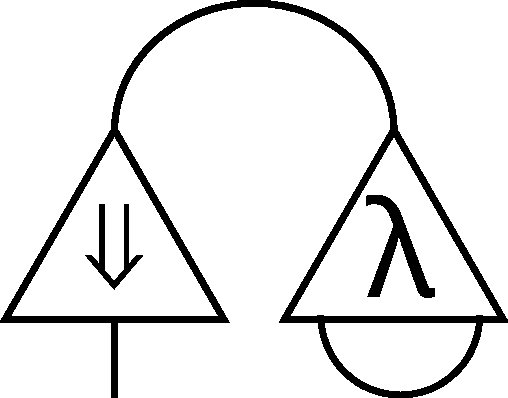
\includegraphics[width=0.5\linewidth]{figures/ins_graph.pdf}
            \end{center}

            Текстовое представление
            \[\big\langle x \mid{} \Downarrow(x) \bowtie \lambda(y, y) \big\rangle\]
        \end{column}
    \end{columns}

\end{frame}

\begin{frame}
    \frametitle{Метрики исполнения}

    \begin{columns}
        \begin{column}{0.45\linewidth}
            Получаемые метрики позволяют отвечать на вопросы
            \begin{itemize}
                \item Сколько операций потребовалось для вычислений?
                \item Какое ускорение можно получить при параллельном исполнении программы?
                \item Сколько \enquote{ядер} ускорителя может использовать программа?
            \end{itemize}
        \end{column}
        \begin{column}{0.5\linewidth}
            \begin{figure}
                \begin{center}
                    \includegraphics[width=\linewidth, page=2]{figures/Figures_cropped.pdf}
                \end{center}
                \caption{Оценка ускорения при использовании параллельности на итеративном факториале}
            \end{figure}
        \end{column}
    \end{columns}

\end{frame}

\begin{frame}
    \frametitle{Результаты}
    В рамках выпускной квалификационной работы были достигнуты следующие результаты
    \begin{enumerate}
        \item Реализован интерпретатор модельного ML-подобного языка со стратегий call-by-need
        \item Реализован транслятор чистого $\lambda$-исчисления в \INs{} в стратегии call-by-value
        \item Реализован интерпретатор \INs{} на основе абстрактной машины с возможностью сбора метрик исполнения
    \end{enumerate}

    \vspace{1em}

    Исходный код находится в репозитории: \url{https://github.com/Lamagraph/interaction-nets-in-fpga}

    Имя коммитера: \texttt{WoWaster}, номера Pull Request: 20, 23, 31, 33, 35, 37, 38
\end{frame}

\appendix

\begin{frame}
    \frametitle{Формальное определение Interaction Nets I/II}

    \begin{columns}[totalwidth=\textwidth]
        \begin{column}{0.6\linewidth}
            \begin{itemize}
                \item $\Sigma$~--- множество символов
                \item Помеченная символом из $\Sigma$ вершина~--- \textit{агент}
                \item Связи между агентами~--- \textit{провода}
                \item Места соединения агентов проводами~--- \textit{порты}
                \item Каждый агент имеет арность $\ar$
            \end{itemize}
        \end{column}
        \begin{column}{0.4\linewidth}
            \begin{center}
                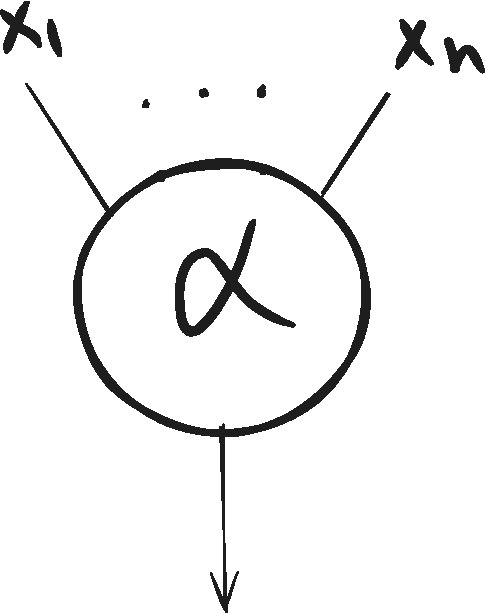
\includegraphics[width=0.3\linewidth]{figures/in_agent.pdf}
            \end{center}
        \end{column}
    \end{columns}
    \begin{itemize}
        \item Если $\alpha \in \Sigma$ и $\ar(\alpha) = n \in \N$, то у $\alpha$ имеется $n+1$ портов: $n$ \textit{дополнительных} и один выделенный~--- \textit{главный}.
    \end{itemize}

\end{frame}

\begin{frame}
    \frametitle{Формальное определение Interaction Nets II/II}

    \begin{itemize}
        \item \textit{Сеть}~--- неориентированный граф с символами из $\Sigma$ в его вершинах
        \item Ребра соединяют порты вершин, в каждый порт приходит не более одного ребра
        \item Порт не соединенный ни с одним ребром~--- \textit{свободный}, множество таких портов~--- \textit{интерфейс}
        \item Пара агентов $(\alpha, \beta) \in \Sigma \times \Sigma$, соединенных своими главными портами,~--- \textit{активная пара}
        \item Правило $((\alpha, \beta) \Longrightarrow N)$ заменяет активную пару $(\alpha, \beta)$ на сеть $N$.
        \item Для каждой пары агентов существует не более одного правила редукции, при этом в процессе редукции интерфейс сохраняется
    \end{itemize}

\end{frame}

\begin{frame}{Interaction Nets}

    \begin{center}
        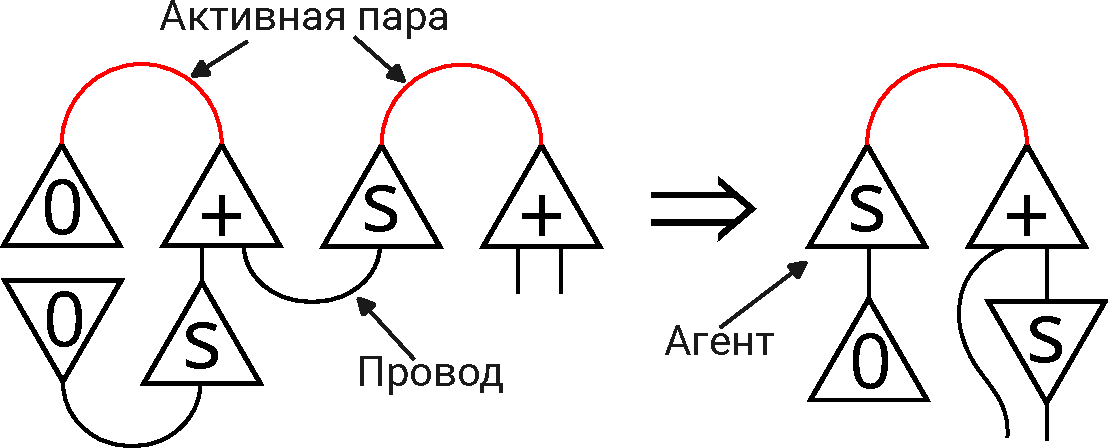
\includegraphics[width=\textwidth]{figures/in_talk.pdf}
    \end{center}

\end{frame}

\begin{frame}
    \frametitle{Схема трансляции\footnote[frame]{По материалам Sinot F.-R. Call-by-Name and Call-by-Value as Token-Passing Interaction Nets // Typed Lambda Calculi and Applications Lecture Notes in Computer Science. / под ред. P. Urzyczyn. Berlin, Heidelberg: Springer Berlin Heidelberg, 2005. С. 386–400.}}

    Пусть $\mathcal{T}(\cdot)$~--- трансляция

    \begin{description}
        \item[Переменные] Переменные представляются проводами, поскольку рассматриваются только замкнутые термы

    \end{description}
    \begin{onlyenv}<1>
        \begin{columns}[totalwidth=\textwidth]
            \begin{column}{0.6\linewidth}
                \begin{description}
                    \item[Применение] Для применения $\mathcal{T}(t\ u)$ генерируется агент $a$, а к его портам подключаются результаты $\mathcal{T}(t)$ и $\mathcal{T}(u)$.
                          Если множество свободных переменных $t$ и $u$ не пусто, то для общих переменных генерируются агенты-дупликаторы $c$
                \end{description}
            \end{column}
            \begin{column}{0.4\linewidth}
                \begin{center}
                    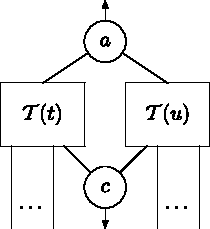
\includegraphics[width=0.5\linewidth]{figures/sinot_app.pdf}
                \end{center}
            \end{column}
        \end{columns}
    \end{onlyenv}

    \begin{onlyenv}<2>
        \begin{columns}[totalwidth=\textwidth]
            \begin{column}{0.6\linewidth}
                \begin{description}
                    \item[Абстракция] Для абстракции $\mathcal{T}(\lambda x.t)$ генерируется агент $\lambda$, правый порт которого связывается с $\mathcal{T}(t)$, а левый с проводом, соответствующим $x$
                \end{description}
            \end{column}
            \begin{column}{0.4\linewidth}
                \begin{center}
                    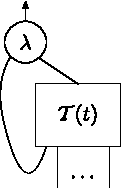
\includegraphics[width=0.4\linewidth]{figures/sinot_abs_1.pdf}
                \end{center}
            \end{column}
        \end{columns}
    \end{onlyenv}

    \begin{onlyenv}<3>
        \begin{columns}[totalwidth=\textwidth]
            \begin{column}{0.6\linewidth}
                \begin{description}
                    \item[Абстракция] Для абстракции $\mathcal{T}(\lambda x.t)$ генерируется агент $\lambda$, правый порт которого связывается с $\mathcal{T}(t)$, если $x$ не содержится в $t$, то генерируется агент-уничтожитель $\varepsilon$
                \end{description}
            \end{column}
            \begin{column}{0.4\linewidth}
                \begin{center}
                    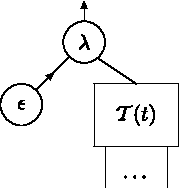
\includegraphics[width=0.5\linewidth]{figures/sinot_abs_2.pdf}
                \end{center}
            \end{column}
        \end{columns}
    \end{onlyenv}
\end{frame}

\end{document}
